\documentclass[11pt,leqno]{article}
\usepackage[polish]{babel}
%\usepackage[OT4]{polski}
\usepackage[utf8]{inputenc}
\usepackage[T1]{fontenc}
\frenchspacing
%\usepackage{indentfirst}
\usepackage{listings}
\usepackage{framed}
\usepackage[textwidth=16cm,textheight=24cm]{geometry}
\usepackage{graphicx}
\usepackage{hyperref}
%\graphicspath{{img\\}}

\usepackage{subfig}
\setlength\fboxsep{0pt}
\setlength\fboxrule{0.5pt}

\newcommand{\myimage}[3]{
  \begin{figure}[h!]
    \centering
      \includegraphics[scale=#1]{#2}
  \caption{#3}
  \end{figure}
}

\usepackage{float}
\floatstyle{boxed} 
\usepackage{wrapfig}


\title{\LARGE Licencjacki projekt programistyczny 2011 \\ 
       \ \\
       Program do wykonywania obliczeń statystycznych związanych z grą go \\ 
       \ \\
       Motywacja dla projektu }

% TODO autor wieksza czcionka

\author{Wojciech Jedynak}
\date{Wrocław, \today}

% \newtheorem{rys}{Rysunek}

\begin{document}

\maketitle 

\thispagestyle{empty}
\tableofcontents

\newpage


\section{Wprowadzenie do gry go}

\subsection{Historia i zasady}

Go jest strategiczną grą planszową pochodzenia chińskiego. Należy zarówno do jednych z nastarszych gier znanych 
ludzkości (niektórzy ocenieją jej historię na około 4 tysiące lat), jak i do najtrudniejszych i najbardziej złożonych.
Liczba możliwych gier jest szacowana na nawet $ 10^{750} $, a średnio w każdej sytuacji gracz ma do wyboru około 200 możliwości.
Bardzo trudno napisać program komputerowy, który grałby dobrze w go. 

Go jest grą dla dwóch graczy. Rogrywka toczy się na kwadratowej planszy przeciętej 19 liniami poziomymi i 19 liniami pionowymi 
tworzącymi 361 przecięć. Aby ułatwić naukę gry  początkującym, używa się również mniejszych plansz, o rozmiarach 9x9 oraz 13x13. 

Na samym początku rozgrywki plansza jest pusta, następnie gracze naprzemiennie kładą na wolnych przecięciach swoje pionki, 
zwane tutaj kamieniami. Gracz, który zaczyna całą partię używa kamieni czarnych, jego przeciwnik ma kamienie białe.

\begin{figure}[h!]
  \centering
  \subfloat[Tradycyjny japoński zestaw do gry w Go: kamienie (często wykonywane z muszli), plansza i pojemniki na kamienie.]
   {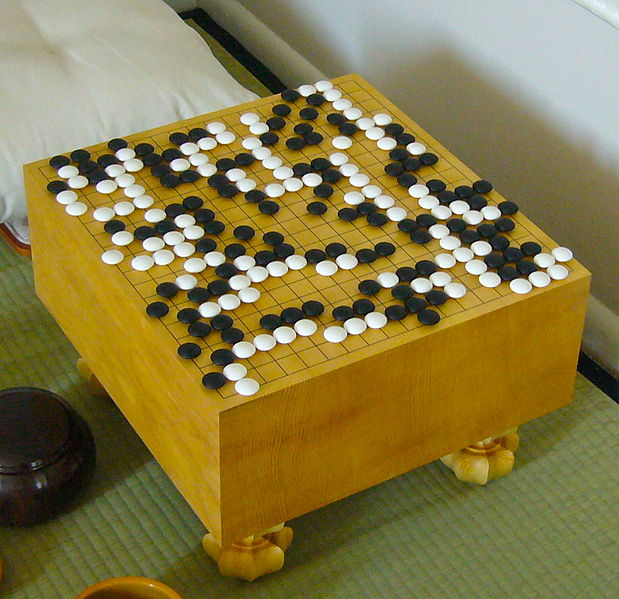
\includegraphics[width=0.4\textwidth]{619px-FloorGoban.JPG}}
  \hspace{0.5cm}                
  \subfloat[Plansza o oficjalnych rozmiarach (19 x 19)]{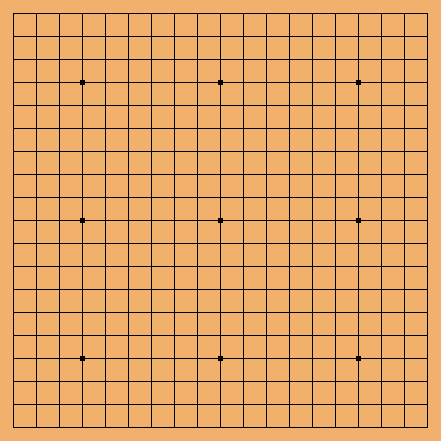
\includegraphics[width=0.4\textwidth]{19.png}}
  %\caption{Pictures of animals}
  
  \subfloat[Plansza pośrednia między 9x9 a 19x19: rozmiar 13x13]
   {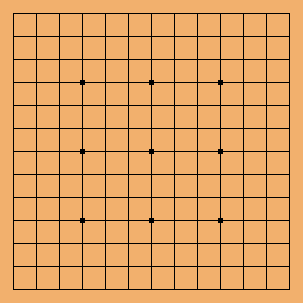
\includegraphics[width=0.4\textwidth]{13.png}}
  \hspace{0.5cm}                
  \subfloat[Najmniejsza plansza używana w praktyce (9x9)]{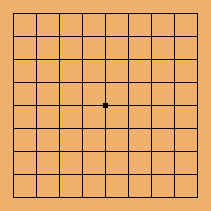
\includegraphics[width=0.4\textwidth]{9.png}}
  %\caption{Pictures of animals}
\end{figure}

\subsection{Popularność gry }

Gra cieszy się ogromną popularnością w Azji wschodniej, w go grają tam setki milionów osób. Na zachodzie gra jest mniej znana, 
ale w bardzo wielu krajach istnieją stowarzyszenia, które zrzeszają miłośników gry. 

W Polsce od ?? roku istnieje Polskie Stowarzyszenie
Go (adres), rozgrywane są Mistrzostwa Polski Kobiet, Par, Juniorów... Istnieje kilkanaście klubów, w których regularnie odbywają
się spotkania goistyczne -- we Wrocławiu funkcjonują dwa kluby: odnośniki! Na liście rankingowej przeważnie znajduje się około 300 do 400 
nazwisk z całego kraju. Aktualnym mistrzem Polski jest ..., zaś na rozgrywanych rokrocznie w Japonii mistrzostwach świata amatorów 
reprezentował Polskę w 2011 roku student Uniwersytetu Wrocławskiego Kamil Chwedyna. 
Kamil zajął rewelacyjne 13 miejsce i otrzymał nagrodę specjalną za 
``swobodę i lekkość stylu'' od głownego sędziego zawodów, którym był sam Masaki Takemiya. 
Takemiya to legendarny japoński gracz zawodowy; odnosił w latach ?? ogromne sukcesy, a jego styl
gry był tak odmienny od tego co uchodziło wówczas za kanon, że jego metodę nazywano ``Kosmicznym go''.

\subsection{Organizacje graczy zawodowych}
W Japonii, Chinach, Korei Południowej i na Tajwanie istnieją organizacje graczy zawodowych, którzy stanowią światową czołówkę konkurującą w 
prestiżowych turniejach o wysokie nagrody pieniężne. Ich poczynaniami fascynują się pasjonaci go z całego świata. Wielu
 zawodowców zamiast na rywalizacji koncentruje się na nauczaniu i odwiedząją turnieje na całym świecie, gdzie analizują 
partie amatorów, rozgrywają gry szkoleniowe i prowadzą wykłady. Wielu zawodowców  wydaje książki z zadaniami treningowymi
 oraz poradniki i leksykony otwarć czy przykładów zagrań o zaskakującej skuteczności. Tylko niewielka cześć z nich jest 
tłumaczona na język angielski, ale kilka wybitnych pozycji jest dostępnych jedynie po angielsku, gdyż opracowali je... zachodni amatorzy!

Co trzeba zrobić, by zostać zawodowcem? Przede wszystkim zacząć naukę gry w bardzo młodym wieku (około 5-8 lat), 
bardzo dużo ćwiczyć (najlepiej pod okiem nauczyciela-zawodowca) i odnieść sukces w organizowanym raz do roku egzaminie, 
co jest wyczynem ekstremalnie trudnym. By podejść bowiem do tego egzaminu należy przejść przez kwalifikacje, następnie 
rozegrać grę z każdym z około 30 innych kandydatów i na koniec uplasować się w najlepszej trójce. Tylko trzy osoby rocznie 
zasilają grono zawodowców...

Czy tylko Azjaci mogą uzyskać licencje zawodową? Niekoniecznie, choć wyjątki są bardzo nieliczne. Do tej pory udało
to się między innymi Rosjanom (Alexander Dinershtein, Svetlana Shiksina), Rumunowi (Catalin Tarjanu) i Amerykaninowi 
(Micheal ...). 

\subsubsection{Polskie akcenty}

Leszek Sołdan (50 lat), który jest czternastokrotnym mistrzem Polski w go, spędził wiele lat w Japonii 
trenując z elitą japońskich kandydatów na zawodowców (jap. insei), jednak nie udało mu się zdać egzaminu. Być może sztuka 
ta uda się w przyszłości Mateuszowi Surmie, który jest aktualnym mistrzem Europy do lat 16 (po raz drugi z rzędu) i jest 
obecnie na drugiej pozycji w polskiej klasyfikacji turniejowej (tuż za Leszkiem Sołdanem).

\subsection{Dalsze informacje}

Więcej informacji o go można znaleźć na stronie http://go.art.pl

\section{Analiza statystyczna otwarć}

\subsection{Wprowadzenie}

Mój dobry kolega i wieloletni popularyzator go we Wrocławiu, Łukasz Fajfrowski opowiedział mi, że znalazł w sieci kolekcję 
kilkuset zapisów parti granych przez zawodowców na planszy 9x9 i postanowił przygotować opracowanie najczęstszych i 
najskuteczniejszych zagrań w początkowej fazie gry. Ponieważ w każdej parti początkowe ustawienie jest identyczne i gra
jest w pełni deterministyczna, posiadanie (i przeanalizowanie) takiej bazy wiedzy pozwoliłoby na:

\begin{enumerate}
\item Podniesienie własnego poziomu gry poprzez wykorzystanie wiedzy i doświadczenia graczy zawodowych
\item Odkrycie, czy pewne zagrania są znacznie lepsze od innych, czy jest to jedynie kwestia indywidualnych preferencji
\end{enumerate}

\subsection{Waga problemu}

W szczególności moglibyśmy się choć trochę przybliżyć do odpowiedzi na jedno z kluczowych pytań: czy w go czarny
 (czyli pierwszy gracz) ma strategię wygrywającą? Jeśli tak, to które ruchy dają pewną wygraną? Od 2007 roku znamy częściową
 odpowiedź dla gry w warcaby \footnote{Schaeffer, Jonathan (2007-07-19). "Checkers Is Solved". Science.}.
 Trudno ocenić kiedy uda się ludzkości wyznaczyć odpowiedz dla gry w szachy. W przypadku go 
sytuacja wygląda tak, że przeanalizowano w pełni grę na planszy 4x4, zaś dla planszy 5x5 wykazano przy pomocy analizy komputerowej,
 że czarny zaczynając od zagrania w środek wygrywa \footnote{http://erikvanderwerf.tengen.nl/5x5/5x5solved.html}. 
Możemy oceniać, że przy nieustającym rozwoju sprzętu i postępach w pracy nad
 algorytmami przeszukującymi drzewo gry uda się w przyszłości uzyskać analogiczne wyniki dla planszy 9x9. Na dzień dzisiejszy,
 większość graczy zawodowych sugeruje, że także dla tej planszy najlepsze jest zagranie w sam środek. Jak zostanie wykazane w 
dalszej części pracy, jest to również najczęściej wybierany ruch przez programy komputerowe.

Należy jednak zwrócić uwagę, że z praktycznego punktu widzenia, plansza 9x9 jest tylko narzędziem treningowym w 
porównaniu z czterokrotnie większą (pod względem liczby przecięć), oficjalną planszą 19x19. Różnice w grze na obu planszach
 nie są jedynie kosmetyczne i ilościowe. Strategia gry na dużej planszy jest niemal zupełnie inna niż na planszy małej. Przykładowo:
Rozpoczęcie w środek na planszy małej to ruch, który ma wpływ na całą planszę. Analogiczne zagranie na planszy 19x19 nie ma takiego 
efektu, gdyż środek jest bardzo odległy od rogów, gdzie najłatwiej rozpocząć budowanie pozycji. Dla dużej planszy zagranie takie jest
 uważane za strategię na specjalne okazje.
Na dużej planszy najskuteczniejszym planem jest niekiedy poświęcenie dużej liczby kamieni, aby uzyskać przewagę w innym miejscu.
 Na mniejszych planszach manewr taki często kończy się przegraną, gdyż strata jest zbyt duża.

Biorąc pod uwagę, że znacznie trudniej jest ocenić jakość ruchu na planszy 19x19, jesteśmy w stanie zrozumieć, dlaczego 
nie ma do tej pory programów, które mogłyby się mierzyć z zawodowcam, ba! nawet z dobrymi amatorami, podczas gdy w przypadku 
planszy 9x9 najlepsze sztuczne inteligencje radzą sobie przyzwoicie w grach z ludźmi (na poziomie amatorskim).

\section{Problemy z ręczną obróbką kolekcji gier}

Podczas ręcznego tworzenia swojego opracowania, Łukasz dopisywał kolejne warianty do jednego pliku SGF, który miał 
zawierać kilkanaście ruchów z każdej parti z dostępnego archiwum, i aktualizował na bieżąco dane statystyczne. Było to bardzo 
czasochłonne, żmudne i wymagało dużej koncentracji. Jednym z powodów tego był fakt, iż należało w pamięci dokonywać normalizacji
 ruchów, aby wziąć pod uwagę symetrie. 

\begin{wrapfigure}{l}{0.3\textwidth}
  \vspace{-20pt}
  \begin{center}
    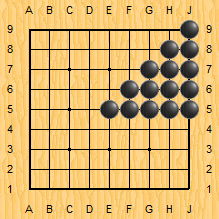
\includegraphics[width=0.28\textwidth]{symetria.png}
  \end{center}
  \vspace{-20pt}
  \caption{15 możliwych sposobów na rozpoczęcie gry, z dokładnością do symetrii \\i obrotów}
  \vspace{-10pt}
\end{wrapfigure}

Na planszy 9x9 mamy do dyspozycji 81 wolnych przecięć, ale z matematycznego punktu widzenia, zagrania w dowolny naróżnik 
(A9, J9, A1, J1) są równoważne z dokładności do obrotu lub symetrii. Jedynie ruch w sam środek jest pod tym względem unikatowy. 
Aby statystyka była poprawna, dwa symetryczne zagrania należy liczyć jako dwa wystąpienia tego samego ruchu! Najmniej podatnym
 na błędy rozwiązaniem wydaje się wybranie pewnego zbioru ruchów, które są parami różne także po uwzględnieniu przekształceń 
geometrycznych. Przykładowy taki zbiór oznaczono na ilustracji obok. Jak widać, ma on 15 elementów. Normalizacja ruchy polega
 więc na znalezieniu równoważnego ruchu, który należy do tych 15 wyróżnionych. Niedogodność, która się z tym wiąże polega na 
tym, że jeśli znormalizujemy pierwszy ruch danej partii, musimy w ten sam sposób przekształcić wszystkie następne ruchy z tej samej gry. 
Przykładowo, jeśli na czarnego F4 biały odpowiedział A6, to nie wystarczy jedynie przekształcić
F4 na F6 - musimy także zmienić A6 na A4.

Widzimy, że cały proces jest nieco zbyt skompikowany \footnote{Szczegółowa analiza, lista potrzebnych przekształceń, 
opis ich własności itp. znajduje się w dokumentacji programisty.}, a cała operacja zbyt żmudna, by wykonywać ją ręcznie dla więcej niż 
kilkunastu gier (statystyczna gra na planszy 9x9 trwa około 50 ruchów), a interesować nas mogą także kolekcje składające się
 z dziesiątek tysięcy partii.

Powyższa analiza pokazuje, że mamy tutaj znakomitą okazję na automatyzację całego procesu za pomocą programu komputerowego. 

\section{Wybór technologii i narzędzi}

\subsection{Analiza techniczna zagadnienia}
Zwróćmy uwagę, że jednym z kluczowych modułów programu do opisanej wyżej analizy będzie moduł przekształceń geometrycznych i
 funkcja normalizująca dany ruch, a następnie całą grę. Błąd logiczny w tym module grozi, że nasze wyniki będą po prostu 
niepoprawne czy sprzeczne. Dobrze byłoby więc użyć narzędzia, które pozwoli nam na operowanie na możliwie wysokim poziomie
 abstracji oraz testowanie funkcji nie tylko dla konkretnych danych, ale na określanie własności na których nam zależy. 
Dodatkowo, potrzebne będzie wsparcie dla bazy danych, serwera HTTP i GUI, gdyż program musi być przetwarzać duże ilości danych
 i musi przezentować wyniki w przystępny dla użytkownika sposób. 

\subsection{Haskell}
Haskell jako język funkcyjny (a więc dobrze wspierający abstracje,
 modularność i poprawność) o otwartym kodzie, posiadający wydajną implementacje (GHC) i dosłownie tysiące dostępnych modułów
 (bibliotek) do przeróżnych zadań zebranych w serwisie Hackage, wydaje się rozwiązaniem optymalnym.

Szczegółowa analiza mocnych stron języka i tego jak przyczyniły się one do powstania projektu znajduje się w dokumentacji programisty.

\section{Odnośniki}
Ilustracje wykorzystane w niniejszym dokumencie pochodzą ze stron \url{http://jeudego.info/?Goban} oraz 
\url{http://en.wikipedia.org/wiki/Go\_(game)}.


\end{document}
